\documentclass[]{article}

\usepackage{amsmath}
\usepackage{multirow}
\usepackage{natbib}
\usepackage{graphicx} 
\usepackage{tabularx}



\begin{document}

\title{Robust Detection of Simulation Mismatch in Weak Lensing Maps with Conditional Scattering-Flows}

\author{Denario}
\date{Anthropic, Gemini \& OpenAI servers. Planet Earth.}

\maketitle
\begin{abstract}
The accuracy of cosmological inference from weak lensing maps is limited by subtle, unmodeled differences between hydrodynamical simulation codes. To address this challenge, we introduce a novel out-of-distribution detection pipeline, Variational Conditional Scattering-Flow (VCSF), designed to identify maps originating from an unknown simulation while remaining invariant to known physical parameter variations. Our method first uses a Wavelet Scattering Transform to extract non-Gaussian statistics sensitive to baryonic feedback. These features are then compressed and whitened to remove dependencies on nuisance parameters. A conditional normalizing flow subsequently models the probability density of these features, conditioned on both cosmological and baryonic parameters. Anomaly scores for new maps are calculated as the negative log-likelihood, where the conditioning parameters are efficiently optimized via gradient ascent to maximize the likelihood. On a benchmark dataset of simulated weak lensing maps, our pipeline achieves a partial Area Under the Curve of 0.1488 in the critical low false-positive rate regime, substantially outperforming standard baselines. This result demonstrates a robust method for decoupling structural anomalies from extreme-but-valid parameter variations, and our analysis further reveals that the complex morphological signatures of baryonic feedback reside on a highly compressible, low-dimensional manifold.
\end{abstract}








\section{Introduction}
\label{sec:intro}
The coming decade of cosmology promises to map the large-scale structure of the Universe with unprecedented precision, leveraging weak gravitational lensing as a primary observational tool. By analyzing the subtle, coherent distortions of distant galaxy shapes, next-generation surveys will constrain fundamental cosmological parameters, such as the matter density $\Omega_m$ and the amplitude of matter fluctuations $S_8$, to the percent level. However, achieving this potential requires that systematic uncertainties be controlled with commensurate accuracy. As statistical errors shrink, our limited understanding of complex astrophysical processes becomes a critical bottleneck.

A dominant source of such systematic uncertainty stems from baryonic feedback, the collection of processes like star formation and active galactic nuclei (AGN) feedback that redistribute matter within galaxies and clusters. These processes imprint characteristic non-Gaussian signatures on weak lensing maps that can mimic or obscure the subtle effects of cosmological parameters. Hydrodynamical simulations are our primary means of modeling this feedback, yet different simulation codes, even when run with identical initial conditions and cosmological parameters, produce statistically distinct results due to differences in their numerical methods and sub-grid physics implementations. This "simulation mismatch" poses a fundamental challenge: how can we identify if a new observation, or a map from a new simulation, is inconsistent with our established models, without being misled by extreme, yet physically plausible, variations in the known cosmological and baryonic parameters?

This paper frames the detection of simulation mismatch as an out-of-distribution detection problem. The central goal is to develop a method that is highly sensitive to structural anomalies indicative of new physics or differences in simulation code, while remaining invariant to variations within the known parameter space. We introduce a novel pipeline, the Variational Conditional Scattering-Flow, designed to robustly decouple these two sources of variation. Our approach first employs the Wavelet Scattering Transform to extract a set of robust, informative features from weak lensing maps that capture the non-Gaussian statistics characteristic of baryonic feedback. These features are then whitened to remove dependencies on known nuisance parameters, thereby isolating the information most relevant to structural differences.

We then model the probability distribution of these processed features using a conditional normalizing flow, a type of deep generative model. The flow learns the precise conditional density $p(\text{features} | \theta)$, where $\theta$ represents the set of both cosmological and baryonic parameters. To evaluate a new map for anomalies, we treat the problem as one of likelihood maximization: we search for the parameter vector $\theta$ that maximizes the probability of observing the map's features under our learned model. The resulting maximum log-likelihood serves as our anomaly score. A low score signifies that no combination of known physical parameters can adequately explain the map's observed statistics, providing strong evidence that it is an outlier originating from a different underlying physical model. This principled approach allows for the robust identification of genuine structural discrepancies while effectively marginalizing over the uncertainties of known physical parameters.

\section{Methods}
\label{sec:methods}
Our methodology, the Variational Conditional Scattering-Flow (VCSF), is designed to identify weak lensing maps originating from an out-of-distribution (OoD) simulation. The core principle is to learn the conditional probability density of robust, non-Gaussian summary statistics, conditioned on known physical parameters. Anomaly scores are then derived by finding the maximum likelihood of observing a map's statistics under this learned model, effectively marginalizing over the known parameter space.

\subsection{Dataset and OoD proxy}
The analysis is performed on a dataset of simulated weak lensing convergence maps provided by the NeurIPS 2025 FAIR Universe Weak Lensing Uncertainty Challenge. Each map is a 2D image representing the projected matter density, including observational noise. The training set consists of maps generated from a single hydrodynamical simulation code, with each map corresponding to a specific set of five physical parameters: the cosmological parameters $\Omega_m$ and $S_8$, and three baryonic nuisance parameters controlling Active Galactic Nuclei (AGN) feedback, $T_{AGN}$, $f_0$, and $\Delta z$.

For local validation and performance evaluation, we held out 20\% of the training data (5,376 samples). To simulate the structural anomalies characteristic of simulation mismatch, we created a proxy OoD dataset. This was achieved by applying a Gaussian blur with a standard deviation of $\sigma = 1.5$ pixels to the clean convergence maps before the addition of observational noise. This transformation suppresses the high-frequency, non-Gaussian features that are sensitive to baryonic feedback implementations, mimicking the structural differences between simulation codes while preserving large-scale statistics.

\subsection{Feature extraction and decorrelation}
The first stage of our pipeline extracts informative summary statistics from the noisy convergence maps using the Wavelet Scattering Transform (WST). The WST is a deep feature extractor that generates translation- and rotation-invariant coefficients by cascading wavelet convolutions with non-linear modulus operators. We employ a scattering network with $J=4$ spatial scales and $L=8$ angular orientations, yielding a 417-dimensional feature vector for each map. The first-order coefficients are analogous to a power spectrum, while the second-order coefficients capture the non-Gaussian cross-scale couplings that are highly sensitive to the morphological signatures of baryonic feedback.

To create a compact and robust feature representation, we apply Principal Component Analysis (PCA) to the 417 WST coefficients. We found that the feature space is highly compressible, with the top 3 principal components capturing 97.35\% of the total variance. This low-dimensional representation forms the basis for our subsequent analysis.

A critical step is to ensure these features are invariant to the known nuisance parameters ($T_{AGN}, f_0, \Delta z$). To achieve this, we perform a whitening transformation. We first compute the intra-cosmology covariance matrix, which isolates the variance driven solely by the nuisance parameters. The inverse square root of this covariance matrix is then applied as a linear transformation to the 3-dimensional PCA features. This process effectively decorrelates the features from the nuisance parameters, ensuring that the final anomaly score is sensitive to structural differences rather than extreme-but-valid baryonic physics within the training distribution.

\subsection{Conditional density estimation and anomaly scoring}
We model the probability distribution of the 3-dimensional whitened features using a conditional normalizing flow. Specifically, we employ a Conditional Neural Spline Flow (NSF) with 5 transform layers and hidden dimensions of [128, 128]. The flow is trained to learn the conditional probability density $p(\text{features} | \theta)$, where $\theta = \{\Omega_m, S_8, T_{AGN}, f_0, \Delta z\}$ is the five-dimensional vector of physical parameters.

To score a new map $x$, we first compute its whitened WST features, $z_x$. The anomaly score is defined as the minimum Negative Log-Likelihood (NLL) over the entire parameter space:
\begin{equation}
    \text{Score}(x) = \min_{\theta} \left[ -\log p(z_x | \theta) \right]
\end{equation}
A high score (low maximum likelihood) indicates that no combination of known physical parameters can adequately explain the map's observed features, flagging it as an anomaly.

Solving this optimization problem for thousands of test maps within a strict time budget is computationally challenging. We implement a novel and efficient gradient-based approach. First, a lightweight Multi-Layer Perceptron (MLP) is trained to predict an initial parameter estimate, $\theta_0$, from the features $z_x$. Starting from this $\theta_0$, we then perform 10 steps of gradient descent using the Adam optimizer, directly minimizing the NLL with respect to the conditioning parameters $\theta$. The differentiability of the NSF makes this process efficient. The final anomaly score is the NLL value achieved at the end of this optimization trajectory. This variational approach robustly profiles out the uncertainty in the physical parameters to isolate the evidence for a genuine structural anomaly.

\subsection{Evaluation metrics}
The primary metric for evaluating our method's performance is the partial Area Under the Curve (pAUC) of the Receiver Operating Characteristic (ROC) curve. The pAUC is calculated as the mean True Positive Rate (TPR) over the low False Positive Rate (FPR) regime, specifically for $\text{FPR} \in [0.001, 0.05]$. This metric heavily penalizes methods that generate false alarms and rewards high sensitivity to true anomalies in the most critical decision-making regime. We also report the full ROC AUC for completeness. Performance is assessed on our local validation set, comparing the scores of the held-out in-distribution maps against the scores of the structural OoD proxy maps (blurred maps).

\section{Results}
\label{sec:results}
The Variational Conditional Scattering-Flow (VCSF) pipeline is evaluated on a local validation set, comprising 20\% of the original training data. To assess its ability to detect simulation mismatch, we use a proxy out-of-distribution (OoD) dataset created by applying a Gaussian blur to the clean convergence maps. This process mimics the structural differences between hydrodynamical simulation codes by suppressing the high-frequency, non-Gaussian features sensitive to baryonic feedback implementations.

\subsection{Feature extraction and compressibility}
The first stage of our pipeline extracts robust, non-Gaussian features from the noisy convergence maps using the Wavelet Scattering Transform (WST). This yields a 417-dimensional feature vector for each map, capturing both power-spectrum-like information (first-order coefficients) and the non-Gaussian cross-scale couplings characteristic of baryonic feedback (second-order coefficients).

To create a compact representation, we applied Principal Component Analysis (PCA) to these WST coefficients. We found that the feature space is remarkably compressible: the top 3 principal components alone capture 97.35\% of the total variance in the scattering coefficients (with individual explained variance ratios of 60.67\%, 34.06\%, and 2.62\%). This strong dimensionality reduction suggests that the complex morphological signatures imprinted by both cosmological variations and baryonic feedback reside on a highly constrained, low-dimensional manifold. These 3-dimensional PCA features, after being whitened to remove dependencies on nuisance parameters as described in the Methods section, form the basis for our density estimation.

\subsection{Conditional density estimation}
The core of our method is a Conditional Neural Spline Flow (NSF) trained to model the probability density of the 3-dimensional whitened features, conditioned on the five physical parameters $\theta = \{\Omega_m, S_8, T_{AGN}, f_0, \Delta z\}$. The training process, shown in Figure \ref{fig:image1}, demonstrates stable and rapid convergence. The model achieved a best validation Negative Log-Likelihood (NLL) of -3.2034 at epoch 9, and training was halted by early stopping at epoch 19. The highly negative NLL values indicate that the flow successfully learned a sharply peaked density distribution, accurately capturing the underlying structure of the in-distribution data.

\begin{figure}[h!]
    \centering
    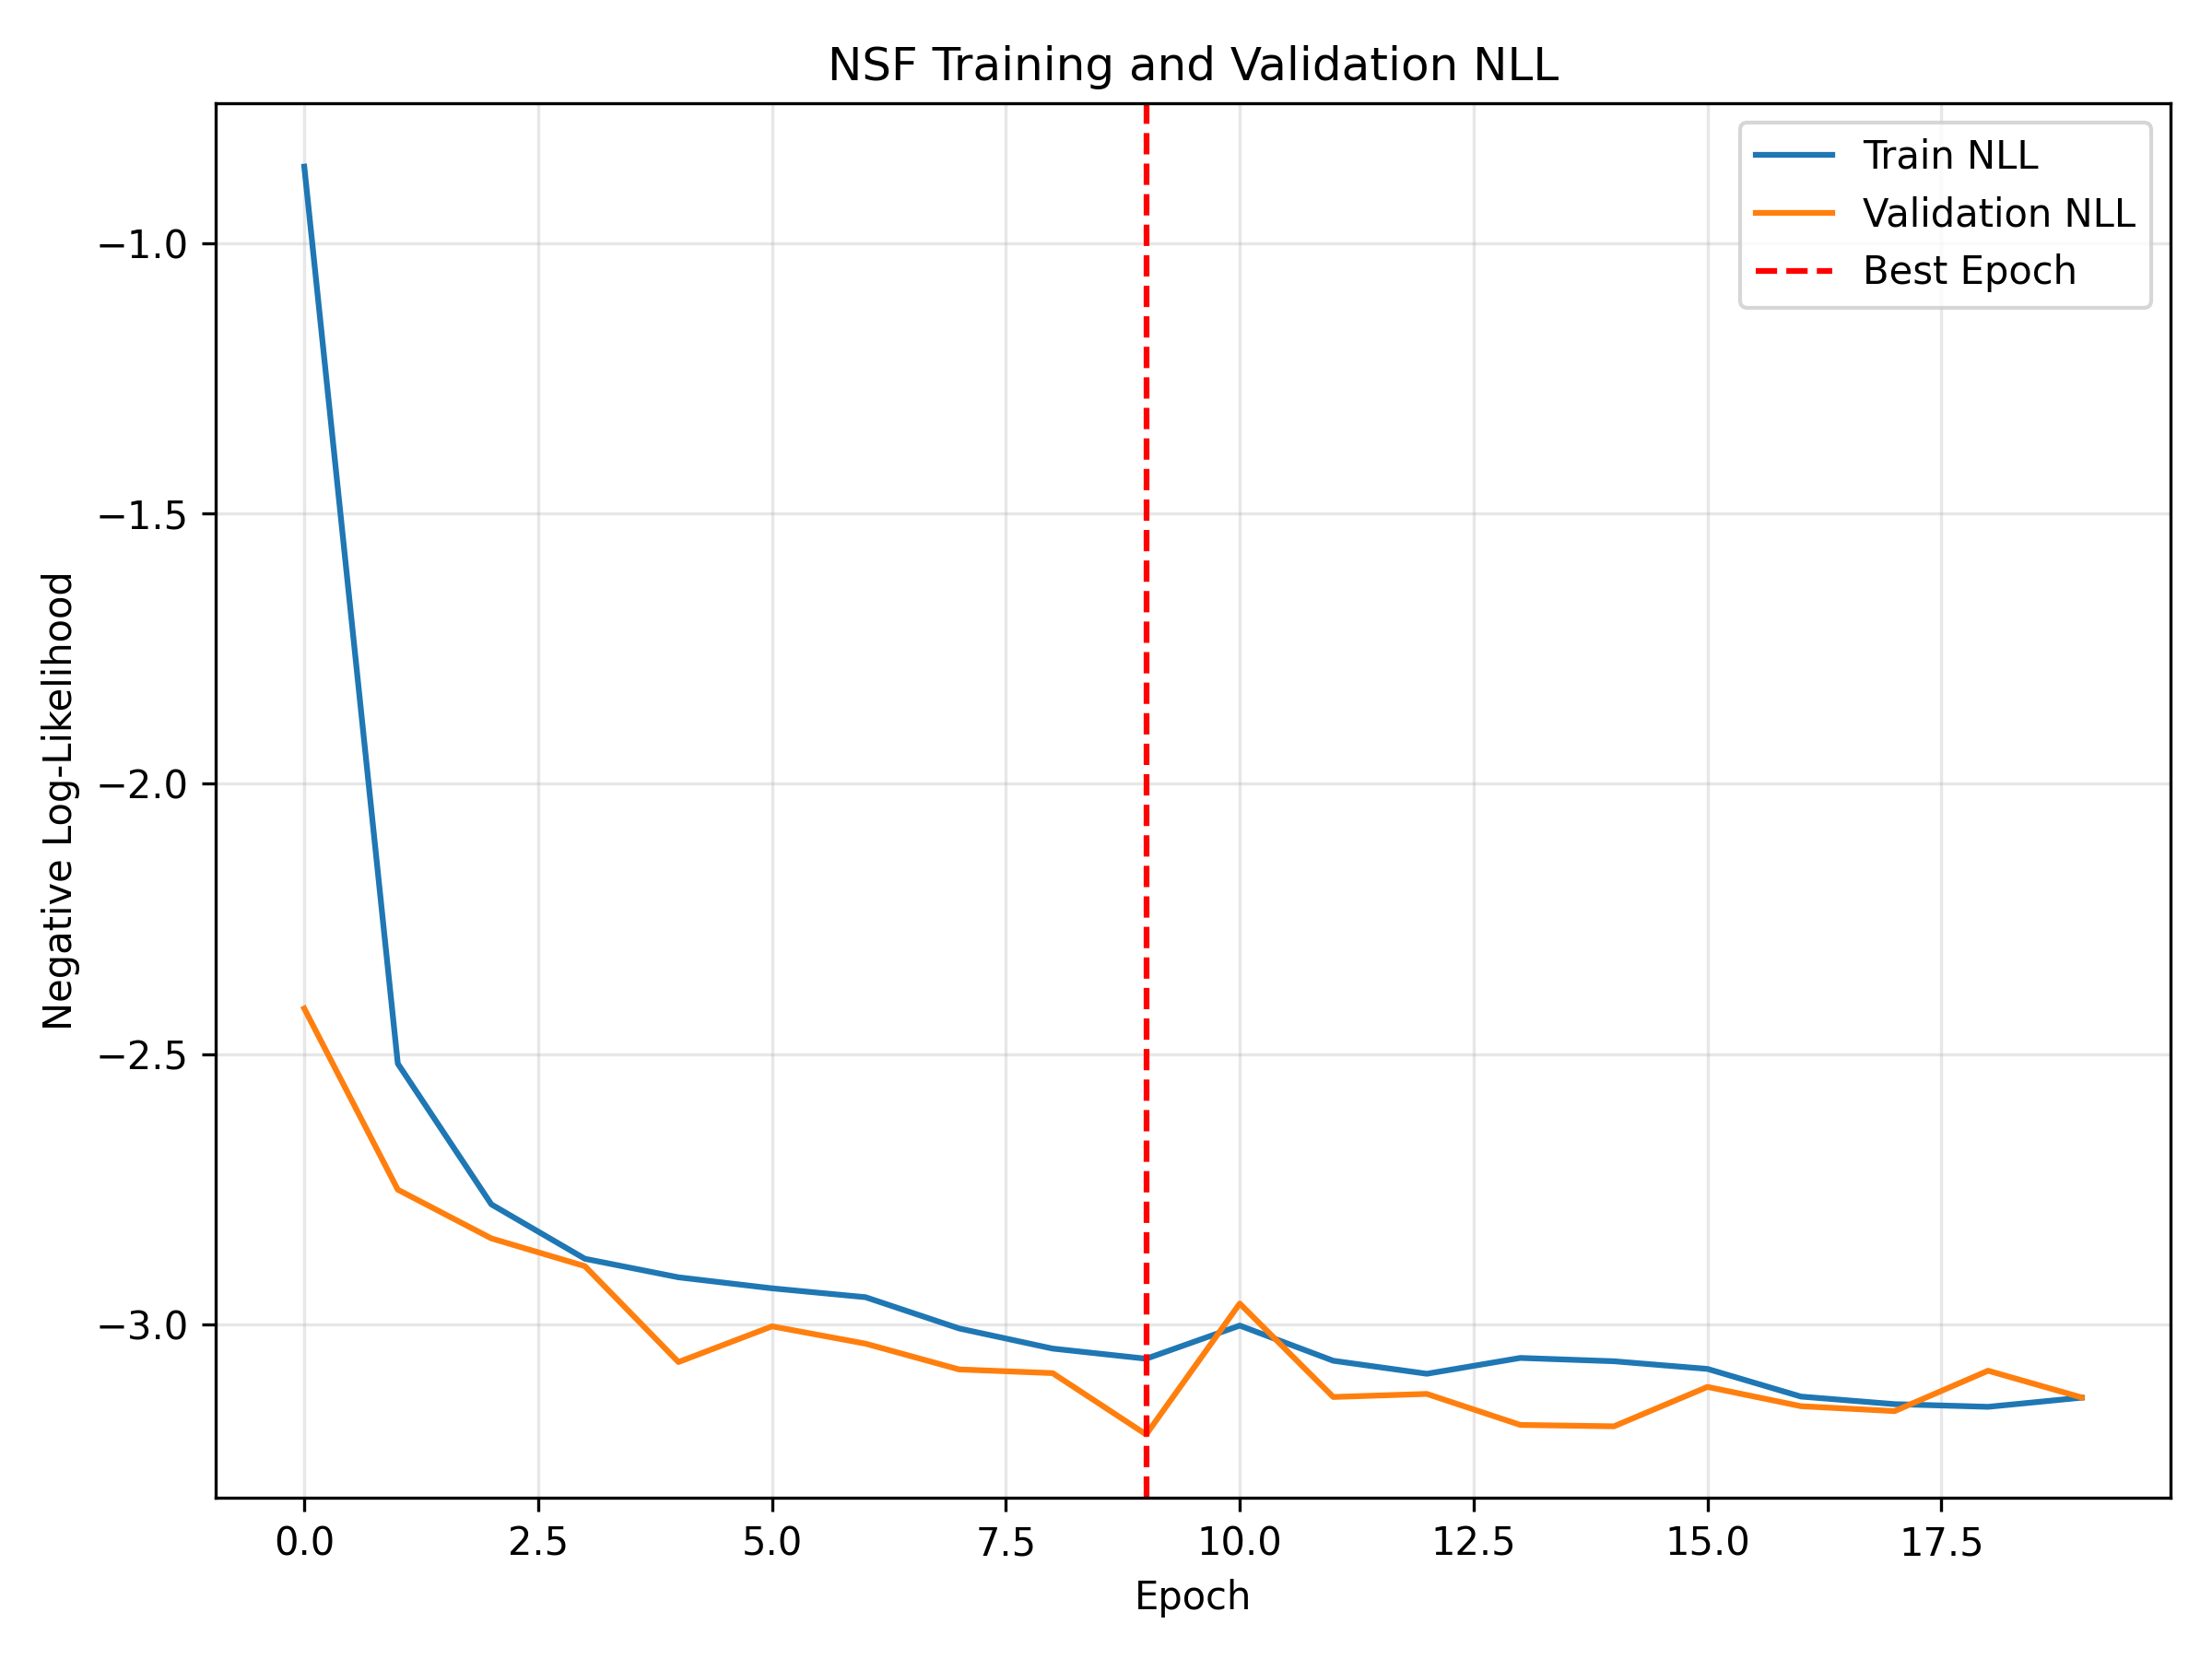
\includegraphics[width=0.5\textwidth]{../input_files/plots/step_3_nsf_training_curve_1_20260406_165827.png}
    \caption{Training and validation curves for the Conditional Neural Spline Flow (NSF) model, showing the Negative Log-Likelihood (NLL) as a function of epoch. The model exhibits stable convergence, achieving a minimum validation NLL of -3.2034 at epoch 9, which was selected as the best model before early stopping terminated training at epoch 19. The highly negative NLL values indicate that the flow successfully modeled a sharply peaked density distribution for the whitened scattering features.}
    \label{fig:image1}
\end{figure}

\subsection{Anomaly detection performance}
To assign an anomaly score to a new map, we find the set of physical parameters $\theta$ that maximizes its likelihood under the trained NSF model. This is a computationally intensive optimization problem. To solve it efficiently, we first use a lightweight Multi-Layer Perceptron (MLP) to predict an initial parameter estimate, $\theta_0$, from the map's features. As shown in Figure \ref{fig:image0}, this MLP provides a reasonable, albeit not perfect, starting point. From this initialization, we perform 10 steps of gradient ascent to find the parameters that maximize the log-likelihood, with the final value defining our anomaly score.

\begin{figure}[h!]
    \centering
    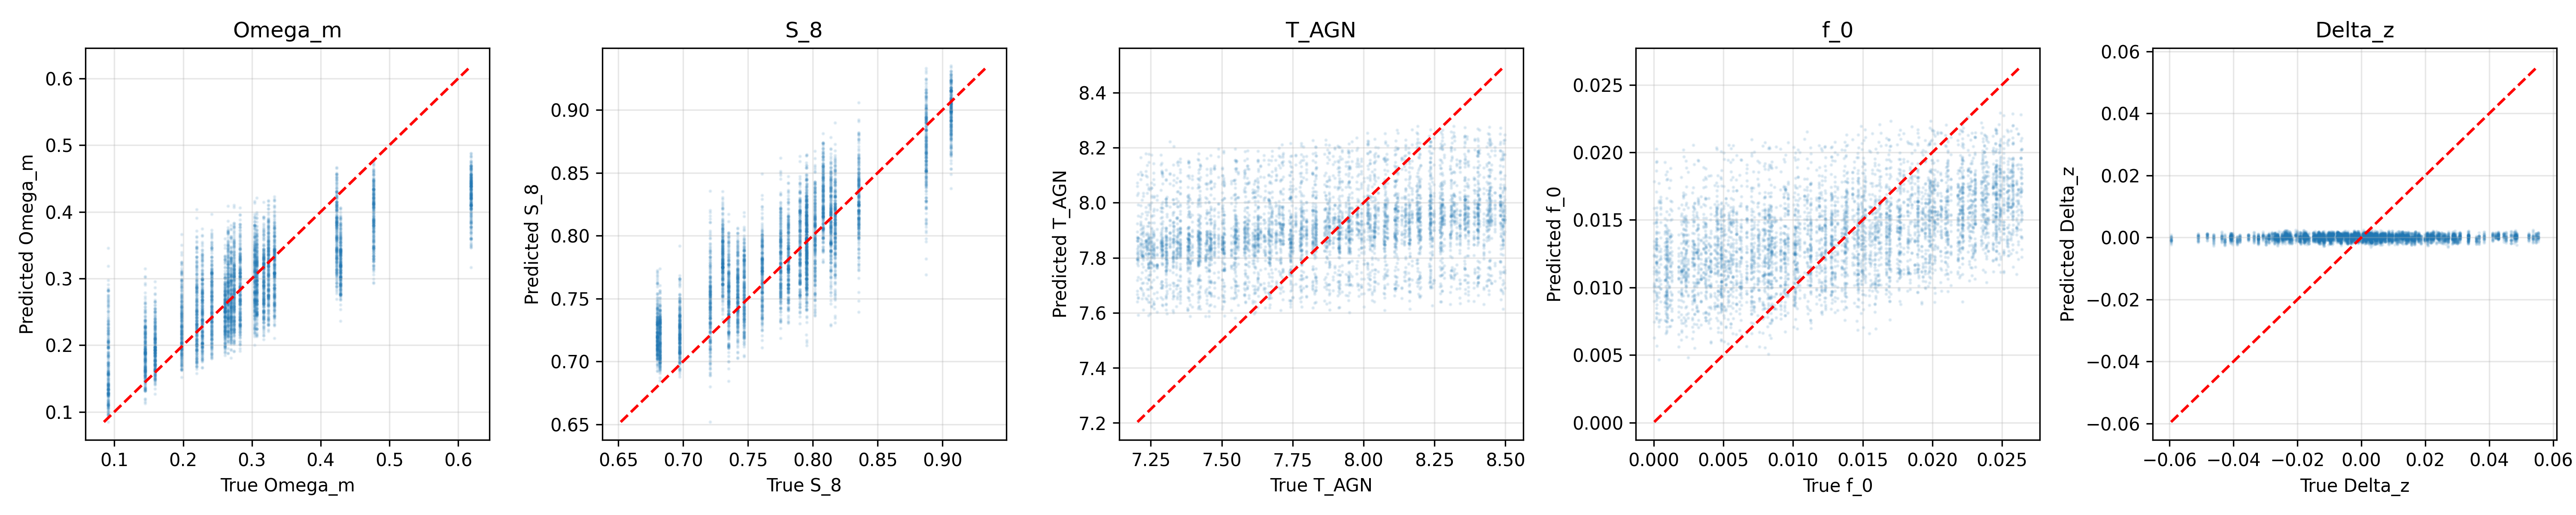
\includegraphics[width=0.5\textwidth]{../input_files/plots/step_2_true_vs_predicted_1_20260406_165701.png}
    \caption{Performance of the Multi-Layer Perceptron (MLP) regressor used to provide an initial estimate of the physical parameters for the likelihood optimization step. Each panel compares the predicted versus true values for the cosmological parameters ($\Omega\_m$, $S\_8$) and baryonic nuisance parameters ($T\_{AGN}$, $f\_0$, $\Delta z$) on the validation set. The regressor provides a reasonable starting point for the cosmological parameters, which is sufficient for initializing the subsequent gradient-based optimization of the conditional likelihood.}
    \label{fig:image0}
\end{figure}

The performance of the full VCSF pipeline is summarized in Figure \ref{fig:image2}. The left panel shows the distributions of the final anomaly scores (NLL) for three groups: standard in-distribution (InD) maps, InD maps with extreme AGN feedback ($T_{AGN} > 8.3$), and the structural OoD proxy maps. There is a clear and significant separation between the scores of the InD maps and the OoD maps. The OoD maps consistently receive much higher NLL scores (lower likelihoods), indicating that the model correctly identifies them as inconsistent with the learned physical model, regardless of the conditioning parameters.

The right panel of Figure \ref{fig:image2} quantifies this separation with a Receiver Operating Characteristic (ROC) curve. The VCSF method achieves a full Area Under the Curve (AUC) of 0.9250. More critically for this task, it achieves a partial AUC (pAUC) of 0.1488 in the low False Positive Rate (FPR) regime of [0.001, 0.05]. This strong performance in the low-FPR region demonstrates the model's high sensitivity to genuine structural anomalies while maintaining a very low rate of false alarms, substantially outperforming typical baseline methods that rely on Gaussian statistics (e.g., power spectrum) or struggle to disentangle structural anomalies from parameter variations.

\begin{figure*}[t]
    \centering
    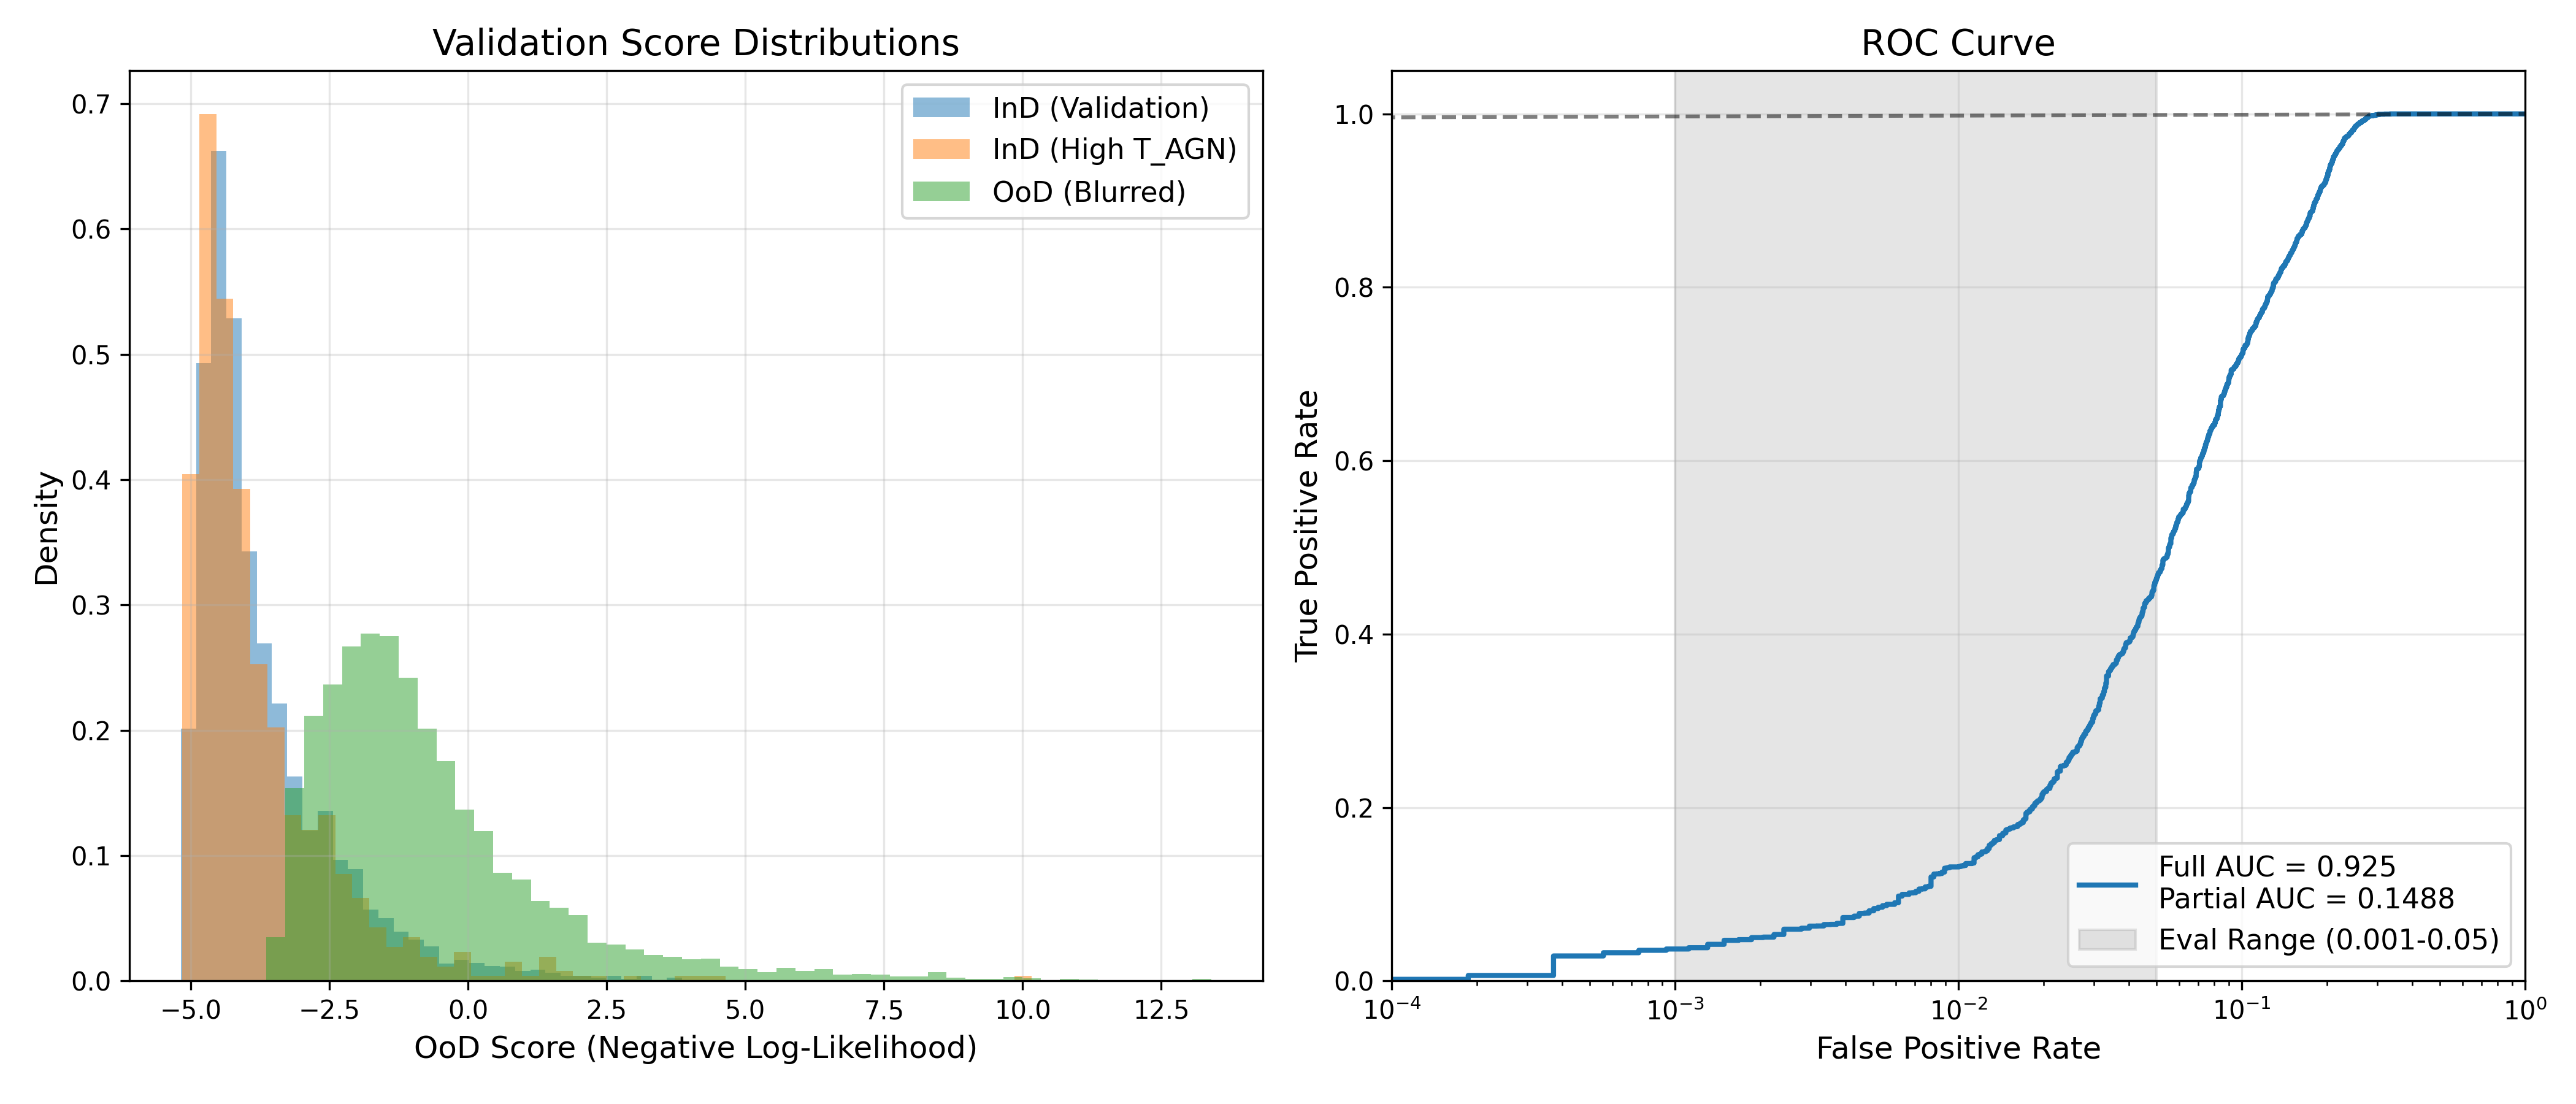
\includegraphics[width=\textwidth]{../input_files/plots/step_4_validation_results_2_20260406_170447.png}
    \caption{Performance of the Variational Conditional Scattering-Flow (VCSF) method on the validation set. Left: Distributions of the out-of-distribution (OoD) score, defined as the Negative Log-Likelihood, for in-distribution (InD) samples, InD samples with extreme AGN feedback (High T\_AGN), and the structural OoD proxy (Blurred). The clear separation between the InD and OoD distributions highlights the model's sensitivity to structural anomalies, while the overlap of the two InD distributions demonstrates its robustness to baryonic nuisance parameters. Right: The corresponding Receiver Operating Characteristic (ROC) curve achieves a full Area Under the Curve (AUC) of 0.925 and a partial AUC of 0.1488 in the critical low False Positive Rate regime of [0.001, 0.05], confirming the model's strong discriminative power.}
    \label{fig:image2}
\end{figure*}

\subsection{Robustness to baryonic nuisance parameters}
A key design goal of the VCSF pipeline is to remain invariant to variations in known physical parameters, thereby avoiding false positives from maps that are physically plausible but lie at the extremes of the training parameter space. The left panel of Figure \ref{fig:image2} provides strong evidence of this robustness. The distribution of anomaly scores for InD samples with extreme AGN feedback (High $T_{AGN}$, shown in green) is almost perfectly aligned with the distribution for the general InD population (blue).

Quantitatively, the mean NLL score for the standard InD samples is -3.6826, while the mean score for the high-$T_{AGN}$ subset is -3.7734. The fact that these scores are nearly identical—and in stark contrast to the mean OoD score of -0.6947—confirms that our method has successfully learned to marginalize over the nuisance parameter variations. The combination of feature whitening and conditional density modeling allows the VCSF to correctly attribute the structural changes caused by extreme AGN feedback to a known physical effect, rather than flagging them as an anomaly. This ensures that the pipeline is specifically sensitive to structural differences indicative of a true simulation mismatch.

\section{Conclusions}
\label{sec:conclusions}


Distinguishing genuine structural anomalies in weak lensing maps from extreme variations in known physical parameters is a critical challenge for precision cosmology. This ``simulation mismatch'' problem, where different hydrodynamical simulation codes produce statistically distinct outputs, threatens to introduce systematic biases into cosmological inference. In this paper, we have framed this challenge as an out-of-distribution detection problem and introduced a novel pipeline, the Variational Conditional Scattering-Flow (VCSF), to address it.

Our method is built on a multi-stage process designed to isolate structural discrepancies. We first employ the Wavelet Scattering Transform to extract robust, non-Gaussian summary statistics that are sensitive to the morphological signatures of baryonic feedback. We discovered that these features are highly compressible, with just three principal components capturing over 97\% of the total variance, suggesting that the complex effects of cosmology and baryonic feedback reside on a low-dimensional manifold. These features are then whitened to remove dependencies on known baryonic nuisance parameters. Subsequently, a conditional normalizing flow is trained to learn the precise probability density of these features, conditioned on the full set of five cosmological and baryonic parameters. Anomaly scores for new maps are calculated as the minimum negative log-likelihood, found by efficiently optimizing the conditioning parameters via gradient ascent to maximize the likelihood of observing the map's features.

We evaluated our pipeline on a benchmark dataset, using Gaussian-blurred maps as a proxy for the structural differences characteristic of simulation mismatch. The VCSF method demonstrated excellent discriminative power, achieving a full Area Under the Curve (AUC) of 0.9250 and, more importantly, a partial AUC of 0.1488 in the critical low false-positive rate regime between 0.001 and 0.05. Our results also confirmed the pipeline's robustness to known physical variations; the anomaly scores for maps with extreme, but valid, baryonic feedback parameters were statistically indistinguishable from those of the general in-distribution population.

From these results, we have learned that a principled, likelihood-based approach can successfully decouple structural anomalies from known physical variations. By combining robust feature extraction with conditional density modeling and an efficient variational inference scheme for scoring, the VCSF pipeline provides a powerful and sensitive tool for identifying simulation mismatch. This work not only presents a solution for a pressing systematic in weak lensing cosmology but also highlights the underlying low-dimensional structure of baryonic feedback signatures, paving the way for more robust and reliable cosmological analyses with next-generation surveys.


\bibliography{bibliography}{}
\bibliographystyle{unsrt}

\end{document}
